\documentclass[11pt,a4paper]{article}
\usepackage[utf8]{inputenc}
\usepackage[T1]{fontenc}
\usepackage[margin=2.5cm]{geometry}
\usepackage{amsmath}
\usepackage{amssymb}
\usepackage{xcolor}
\usepackage{soul}
\usepackage{hyperref}
\usepackage{enumitem}
\usepackage{parskip}
\usepackage{graphicx}
\usepackage{booktabs}
\usepackage{float}
\usepackage{caption}
\graphicspath{{../article/figures/}{../01_compile_manuscript/figures/}{figures/}{./}}

\definecolor{revblue}{RGB}{0,70,140}
\definecolor{revgreen}{RGB}{0,120,60}
\definecolor{revgray}{RGB}{90,90,90}
\definecolor{revred}{RGB}{180,40,40}

\hypersetup{colorlinks=true,linkcolor=revblue,urlcolor=revblue,citecolor=revblue}

% Custom command for reviewer quote box
\newenvironment{revquote}{%
  \begin{quote}\small\itshape\color{revgray}
}{%
  \end{quote}
}

% Custom command for our response
\newcommand{\response}[1]{\par\noindent\textbf{\color{revgreen}Authors' response:} #1\par}

% Custom command for change reference
\newcommand{\changes}[1]{\par\noindent\textbf{\color{revblue}Changes in manuscript:} #1\par}

% Box displaying the exact text now present in the manuscript (so reviewers need not open it)
\newcommand{\msinserted}[1]{\par\smallskip\noindent\textbf{\color{revblue}Exact text now in the manuscript:}\par\smallskip%
\noindent\fbox{\begin{minipage}{0.96\linewidth}\small\itshape #1\end{minipage}}\par\smallskip}

% Status markers
\newcommand{\done}{\color{revgreen}\textbf{[DONE]}}
\newcommand{\inprogress}{\color{revblue}\textbf{[IN PROGRESS]}}
\newcommand{\pending}{\color{revred}\textbf{[PENDING]}}

\title{\textbf{Point-by-Point Response to Reviewers} \\
\large Manuscript: ``Same Prompt, Different Answer: Hidden Non-Determinism in LLM APIs Undermines Scientific Reproducibility'' \\
\large Submitted to \emph{Nature Communications}}

\author{Lucas Rover, Hugo Valadares Siqueira, Eduardo Tadeu Bacalhau, \\
Anibal Tavares de Azevedo, Yara de Souza Tadano \\
Federal University of Technology --- Paraná (UTFPR)}

\date{Revision submitted: May, 2026 --- Original submission: 2026-03-12}

\begin{document}

\maketitle

\section*{Navigation index: reviewer points by topic}

\noindent For convenience, the table below maps each reviewer point to its thematic cluster. Points sharing a row are addressed in cross-referenced responses.

\begin{center}
\renewcommand{\arraystretch}{1.25}
\begin{tabular}{p{6.5cm}p{8.5cm}}
\hline
\textbf{Thematic cluster} & \textbf{Reviewer points} \\
\hline
Deployment-stack reframe (unit of analysis) & R1.1, R3.2 \\
Expansion to coding, math, out-of-AI/ML domains & R1.8, R3.1, R3.4 \\
Field-level reproducibility: textual vs.\ substantive divergence & R1.5, R1.6 \\
Applied PM\textsubscript{2.5} evidence-synthesis impact and validation & R1.9, R3.6 \\
Multi-turn extension to gpt-4o and DeepSeek & R3.3 \\
Mechanism mapping per deployment stack & R3.5 \\
Cloud deployment vs.\ production-serving infrastructure & R1.4 \\
Protocol scope (client-side observability) & R1.10 \\
Concrete divergence examples (Box~1) & R1.12 \\
Provider-specific clarifications (parameters, Perplexity, seeds, captions, docs) & R1.2, R1.3, R1.7, R1.11, R1.13, R1.14, R1.15 \\
\hline
\end{tabular}
\end{center}

\noindent Co-reviewer R2 (Early Career Researcher training) provided no independent comments.

\newpage
%==============================================================
\section*{Response to Reviewer 1}
%==============================================================

We thank Reviewer~1 for the comprehensive and unusually constructive review. The two strengths the reviewer identified --- the three-level reproducibility framework and the temperature-paradox observation --- are central to the contribution we wished to make, and we are grateful that they were recognised. The fifteen substantive issues the reviewer raised have led to substantial improvements; each is addressed individually below.

%--------------------------------------------------------------
\subsection*{R1.1 --- Framing: APIs and infrastructure stacks, not models}
%--------------------------------------------------------------

\begin{revquote}
While the paper frames the testing as testing of different models, what is being tested is actually APIs and associated infrastructure stacks. Specifically, the same model served by a different API may have different degrees of non-determinism. Could this framing be corrected?
\end{revquote}

\response{We agree entirely. This is the central conceptual observation of the review and we have restructured the manuscript accordingly. We now define a \emph{deployment stack} as the tuple (model weights, provider, serving infrastructure, API layer) and treat it as the unit of analysis throughout. Each component of the tuple can independently introduce variation, and the same model weights served by two different stacks constitute two distinct experimental objects for reproducibility purposes. The Together AI quasi-isolation result --- in which the same LLaMA~3 8B weights served via two different stacks produced markedly different reproducibility profiles --- is now positioned as the direct empirical evidence that the stack, not the model, carries the variation.} \done

\changes{
\begin{itemize}[leftmargin=*]
  \item \textbf{Abstract} (lines 62--67): inserted ``deployment stacks'' tuple definition; substituted ``API-served models'' $\rightarrow$ ``API-served stacks''; clarified the quasi-isolation as same weights served by two different stacks.
  \item \textbf{Introduction:} new paragraph anchoring the deployment-stack concept, and the third contribution rewritten to emphasise ``same weights served via two stacks''. The exact inserted text reads:
  \msinserted{A central conceptual point underlies our analysis: when a researcher queries an LLM through an API, the experimental object is not a model in the abstract sense but a deployment stack, the tuple (model weights, provider, serving infrastructure, API layer). The same weights served by two different stacks can yield two different reproducibility profiles, because each component of the tuple can independently introduce variation through tensor parallelism, mixed-precision accumulation, dynamic batching, or post-processing. We therefore frame results per stack rather than per model: identifiers such as ``GPT-4'' refer throughout to the full deployment stack served by the provider at the time of measurement, not to a model abstraction independent of how it is served. [\ldots] Third, we demonstrate that cloud deployment \emph{per se} does not cause non-determinism: the same LLaMA~3 8B weights served via two stacks (local Ollama versus Together AI's cloud endpoint) achieve near-identical exact match rates. This implicates production-infrastructure complexity---tensor parallelism, speculative decoding, dynamic batching---rather than the cloud medium itself, and confirms that the deployment stack, not the model in isolation, is the carrier of variation.}
  \item \textbf{Results §1 heading and lead} (lines 115, 117): renamed and updated terminology consistently.
  \item \textbf{Table~1} (label \texttt{tab:main}): caption rewritten; column header ``Model / Deployment'' $\rightarrow$ ``Deployment stack (weights) / Class''; cross-reference to the deployment-stacks Methods subsection added.
  \item \textbf{Figures 1, 2, 5 captions} (lines 230--235, 271--276, 315--318): ``model deployments'' $\rightarrow$ ``deployment stacks''; ``local models / API models'' $\rightarrow$ ``local stacks / API stacks''.
  \item \textbf{Methods --- new subsection ``Unit of analysis: deployment stacks''} inserted before the (renamed) ``Deployment stacks evaluated'' subsection. The exact inserted text reads:
  \msinserted{We define a \emph{deployment stack} as the tuple (model weights, provider, serving infrastructure, API layer). The same model weights served by two different stacks constitute two distinct experimental objects for reproducibility purposes, since each component of the tuple can independently introduce variation: weights through quantisation, provider through routing and post-processing, serving infrastructure through tensor parallelism, mixed-precision accumulation, FlashAttention kernels, dynamic batching, and speculative decoding, and the API layer through prompt templating, response truncation, and resolved-version aliasing. This conceptual frame resolves the question of whether observed differences arise from the model itself or from how it is served. The Together AI quasi-isolation probe provides direct evidence: the same LLaMA~3 8B weights served via local Ollama versus Together AI's cloud endpoint produce stacks with measurably different reproducibility profiles, even when the underlying weights are identical. We therefore report results per \emph{stack} rather than per \emph{model}. Throughout the manuscript, identifiers such as ``GPT-4'' refer to the full deployment stack (gpt-4-0613 / OpenAI / production cluster / Chat Completions API) at the time of measurement, not to a provider-independent model abstraction.}
  \item \textbf{Methods --- ``Deployment stacks evaluated''} (line 417 onwards): renamed from ``Models and infrastructure''; entries restructured as full tuples (e.g., L-LLaMA3 = (LLaMA~3 8B Q4 / local Ollama / single-GPU Apple~M4 / \texttt{/api/generate} endpoint)).
  \item \textbf{Discussion:} new paragraph after the Together AI quasi-isolation discussion. The exact inserted text reads:
  \msinserted{A direct consequence is that the \emph{deployment stack}, not the abstract model, is the carrier of variation in LLM-based research. The same LLaMA~3 8B weights yield near-perfect reproducibility under one stack (local Ollama) and substantially lower reproducibility when wrapped in a different cloud-serving stack; conversely, two different sets of weights served by stacks of comparable complexity (GPT-4 and Claude) show qualitatively similar reproducibility profiles. This reframes the methodological recommendation: research and regulatory documentation that names ``the model'' should instead identify the deployment stack as a tuple of weights, provider, serving infrastructure, and API layer. Without that specification, ``using GPT-4'' or ``using Claude'' is under-specified for reproducibility purposes, because the same nominal model served through different stacks can produce materially different outputs and stability profiles.}
\end{itemize}
}

%--------------------------------------------------------------
\subsection*{R1.2 --- Comparability across providers with different parameter exposure}
%--------------------------------------------------------------

\begin{revquote}
The authors write that ``all providers expose the same user-facing `deterministic' parameters (temperature zero, fixed seed where supported)'' yet later note that the settings each specific API offers vary. How does this affect comparability?
\end{revquote}

\response{The reviewer correctly identifies that providers expose overlapping but not identical parameter surfaces. The deterministic configuration we set is the maximum each provider exposes for that purpose. We now make this explicit. Specifically: temperature zero is universally exposed; the seed parameter is supported by OpenAI (advisory) and Gemini, absent from Anthropic, and not exposed by DeepSeek's OpenAI-compatible Chat Completions interface or by Perplexity Sonar. Our \texttt{seed\_status} Run-Card field already records this asymmetry per stack (\texttt{sent}, \texttt{logged-only-not-sent}, or \texttt{not-supported}). What is comparable across stacks is therefore not parameter \emph{equality} but the operational claim that we used the maximum determinism configuration each provider documents, with the precise per-stack parameter set explicit in Supplementary §S4 and the Run Card.} \done

\changes{Methods §``Deployment stacks evaluated'' now lists per-stack parameter exposure explicitly, and Supplementary §S4 gains an introductory ``Comparability across providers'' paragraph. The exact inserted text reads:}
\msinserted{Providers expose overlapping but not identical parameter surfaces. What is comparable across stacks is therefore not parameter \emph{equality} but the operational claim that we used the \emph{maximum determinism configuration each provider documents}: temperature zero is universally exposed; the seed parameter is supported by OpenAI (advisory) and Gemini, absent from the Anthropic Messages API surface, and not exposed by DeepSeek's OpenAI-compatible Chat Completions interface or by Perplexity Sonar. Our \texttt{seed\_status} Run Card field records this asymmetry per stack as \texttt{sent}, \texttt{logged-only-not-sent}, or \texttt{not-supported}. The precise per-stack parameter set for every payload is in the listings below.}

%--------------------------------------------------------------
\subsection*{R1.3 --- Perplexity Sonar's search-augmented architecture (line 103)}
%--------------------------------------------------------------

\begin{revquote}
Line 103 states that ``Perplexity Sonar's particularly low reproducibility reflects its search-augmented architecture, where real-time web retrieval introduces an additional source of variation'' --- it is unclear whether this claim is directly supported by the paper's experiments. If not, the statement should either be supported by appropriate citation or explicitly framed as informed speculation.
\end{revquote}

\response{The reviewer is correct that this claim is not directly tested by an isolation experiment in our study. We have reframed it as an informed hypothesis with citations to Perplexity's public Sonar documentation and to the broader literature on retrieval-augmented generation variability. The reformulated passage now reads:}
\msinserted{Perplexity Sonar's particularly low reproducibility is consistent with its publicly documented search-augmented architecture [perplexitysonar2024], in which each query triggers real-time retrieval over the live web before generation. A plausible mechanism is that variability in the retrieved document set compounds with model-internal non-determinism: the foundational retrieval-augmented generation (RAG) framework [lewis2020rag] treats retrieval as a stochastic component conditioned on a non-stationary corpus, and recent work documents that retrieval variability can produce divergent downstream generations even under fixed model parameters [gao2024rag]. We did not perform a controlled retrieval-isolation experiment for Sonar (the index is not user-accessible), so this mechanism is offered as an informed hypothesis rather than a demonstrated cause.}
\done

\changes{Results §``Non-determinism varies substantially across providers'' --- Perplexity passage rewritten. Three references are added; full details are provided here so they can be consulted without opening the manuscript:
\begin{itemize}[leftmargin=*]
  \item \textbf{[lewis2020rag]} Lewis, P. \emph{et al.} Retrieval-augmented generation for knowledge-intensive NLP tasks. \emph{Advances in Neural Information Processing Systems} \textbf{33}, 9459--9474 (2020). \url{https://arxiv.org/abs/2005.11401}
  \item \textbf{[perplexitysonar2024]} Perplexity AI. Sonar API: real-time web search for LLMs. Official documentation, \url{https://docs.perplexity.ai} (accessed 2026).
  \item \textbf{[gao2024rag]} Gao, Y. \emph{et al.} Retrieval-augmented generation for large language models: a survey. Preprint (2024). \url{https://arxiv.org/abs/2312.10997}
\end{itemize}}

%--------------------------------------------------------------
\subsection*{R1.4 --- Cloud deployment vs.\ production serving infrastructure}
%--------------------------------------------------------------

\begin{revquote}
Line 110 states that ``A natural hypothesis is that cloud deployment itself (network latency, load balancing, shared hardware) causes the non-determinism'', while line 120 states ``The variability observed in GPT-4, Claude, and Gemini is instead consistent with the complexity of their production serving infrastructure''. The distinction between ``cloud deployment itself'' and ``production serving infrastructure'' is currently fuzzy and would benefit from clearer distinction. Listing facets of cloud deployment and known sources of non-determinism is helpful. However, it is not clear that it is comprehensive enough to support the strong conclusions being drawn. What additional factors might be at play in both cloud infrastructure and inference infrastructure?
\end{revquote}

\response{We thank the reviewer for pressing this point; the distinction is indeed underspecified. We have added a new opening paragraph to Methods §``Sources of non-determinism in distributed inference'' that explicitly distinguishes the two factor classes: ``\emph{Cloud deployment factors} are those intrinsic to running a model on hardware accessed over a network: round-trip latency, request routing across geographically distributed endpoints, shared physical hardware, and multi-tenancy isolation. \emph{Production serving infrastructure factors} are specific design choices in the LLM inference stack: tensor parallelism with non-deterministic all-reduce, FlashAttention kernel non-determinism, dynamic batching with continuous request scheduling, speculative decoding fast-paths, mixed-precision BF16/FP16 accumulation, and prefix-caching state across requests.'' The Together~AI quasi-isolation probe controls for the first class (the request still traverses the network, hits a multi-tenant cluster) while differing in serving-infrastructure complexity from the local single-GPU baseline; that this configuration achieves near-local reproducibility is what licenses the inference that the gap originates in serving infrastructure rather than cloud deployment per se. This is now stated explicitly in the new paragraph.} \done

\changes{Methods §``Sources of non-determinism in distributed inference'' --- new opening paragraph explicitly disambiguating the two factor classes, with the Together~AI result invoked to license the inferential bridge (see also the new mechanism-mapping table, R3.5). The exact inserted text reads:}
\msinserted{It is useful to distinguish two classes of factor that are often conflated in discussions of API reproducibility. \emph{Cloud deployment factors} are those intrinsic to running a model on hardware accessed over a network: round-trip latency, request routing across geographically distributed endpoints, shared physical hardware, and multi-tenancy isolation. \emph{Production serving infrastructure factors} are specific design choices made by LLM-serving stacks to maximise throughput and latency efficiency at scale: tensor parallelism, FlashAttention kernel non-determinism, dynamic batching with continuous request scheduling, speculative decoding fast paths, mixed-precision accumulation, and token-level prefix caching across requests. Our Together AI quasi-isolation result shows that the first class alone does not preclude reproducibility---the same LLaMA~3 8B weights served by a cloud endpoint approach near-local EMR. The non-determinism observed for proprietary stacks is therefore consistent with the second class: production serving infrastructure complexity, not the cloud medium itself.}

%--------------------------------------------------------------
\subsection*{R1.5 --- Field-level analysis: textual vs substantive divergence}
%--------------------------------------------------------------

\begin{revquote}
Line 172 states that ``The key result field diverges in 67\% of groups, and method in 57\%''. However, it is not clear whether differences in these fields implies substantive changes in content. Given the reported high semantic similarity and low text edit distance, these differences might reflect minor wording variations than meaningful semantic changes. As currently written, the manuscript appears to conflate opposing claims ``difference is textual not semantic'' and ``difference affects the substantive content'' that need to be resolved.

[\ldots] It would strengthen the argument if the authors computed all metrics on these specific fields to test whether semantic similarity is indeed lower there.
\end{revquote}

\response{We thank the reviewer for identifying this tension and prompting the per-field analysis. We have computed EMR, NED, ROUGE-L, and BERTScore F1 separately for each of the five extracted fields (objective, method, key\_result, model\_or\_system, benchmark) across all stacks. The result resolves the apparent contradiction in a way we did not anticipate and that, on reflection, strengthens the manuscript:

\begin{itemize}[leftmargin=*]
  \item Across the API stacks where outputs actually diverge, the conclusion-relevant fields (objective, method, key\_result) average $\overline{\text{EMR}}=0.455$, while the metadata fields (model\_or\_system, benchmark) average $\overline{\text{EMR}}=0.684$. This is a paired Cohen's $d=+1.41$ effect --- a very large gap.
  \item However, BERTScore F1 is \emph{saturated} across both groups: conclusion-relevant fields average 0.978 and metadata fields 0.979, paired $d=-0.10$ (effectively null).
\end{itemize}

The interpretation is therefore: \emph{BERTScore is structurally unable to discriminate substantive payload divergence from cosmetic textual variation} when one operates on extracted-JSON fields of moderate length. EMR and NED can. The single most striking single-stack illustration is Gemini~2.5~Pro RAG on \texttt{key\_result}, where EMR$=0.10$ (the field changes 90\,\% of the time) while BERTScore F1 remains 0.969. We therefore now argue that the apparent tension the reviewer identified is itself evidence that the three-level reproducibility framework (bitwise $\to$ structural $\to$ semantic) we propose is required: any single metric, including a state-of-the-art semantic similarity metric, would mislead.} \done

\changes{
\begin{itemize}[leftmargin=*]
  \item New \textbf{Supplementary table} (``Per-field reproducibility on structured extraction'', Supplementary §S13) reporting per-stack $\times$ per-field EMR, NED, ROUGE-L F1, and BERTScore F1 with 10\,000-resample percentile bootstrap CIs.
  \item New \textbf{Extended Data Figure} (\texttt{analysis/figures/per\_field\_radar.pdf}) showing per-field BERTScore F1 by stack with a vertical separator between conclusion-relevant and metadata fields, illustrating BERTScore saturation.
  \item Revised \textbf{Results §``Outputs diverge textually but not semantically''} now reports the paired Cohen's $d=+1.41$ EMR gap and the BERTScore null result, and reframes the argument explicitly: BERTScore alone is the wrong instrument for substantive-payload reproducibility, and the three-level framework is necessary precisely because of this.
  \item Discussion now contains the Gemini~2.5~Pro RAG single-stack illustrative case (EMR$=0.10$, BERTScore F1$=0.969$).
\end{itemize}
}

%--------------------------------------------------------------
\subsection*{R1.6 --- Propagation: textual differences affect automated processing}
%--------------------------------------------------------------

\begin{revquote}
``Where outputs are parsed programmatically rather than read by humans, even minor lexical differences can propagate''. Paired with the next paragraph, the point seems to be that these very minor, mostly textual differences can nonetheless affect automated processing of the outputs. This is a key part of the argument, as it prevents the findings from being dismissed as trivial or irrelevant given the high semantic similarity of the results. Clarifying this connection would strengthen the claim that ``non-determinism is therefore not a technical curiosity but a property that interacts with how LLMs are deployed as measurement instruments''.
\end{revquote}

\response{We agree this is the central argumentative bridge that prevents the findings from being dismissed as cosmetic. We have rewritten the paragraph to make the propagation logic explicit: (i)~when outputs feed automated parsers (regex extractors, JSON schema validators, downstream classifiers), even single-character differences in numeric values, dates, or named entities cause divergent extracted records; (ii)~when downstream pipelines aggregate these records into statistics (means, counts, effect sizes), each individual lexical divergence becomes a distinct data-point; (iii)~the per-field EMR drop on \texttt{key\_result} (R1.5) is exactly where this propagation is most consequential, because the \texttt{key\_result} field is what evidence-synthesis pipelines aggregate. The companion PM\textsubscript{2.5} analysis (now expanded) shows this directly: 23 distinct effect estimates appear or disappear from the evidence base depending solely on which run of the LLM is used.} \done

\changes{New Results subsection ``Applied impact in evidence synthesis: an out-of-AI/ML probe'' inserted before the Discussion (manuscript lines 246--264). It explicitly chains the propagation logic from the per-field analysis (R1.5) to the 10-abstract PubMed PM\textsubscript{2.5} extraction probe and, via citation of the companion paper, to the 23 study-level effect estimates that appear or disappear depending on the LLM run.}

%--------------------------------------------------------------
\subsection*{R1.7 --- Figure 1 caption inconsistency (8 vs 5 vs 10 deployments)}
%--------------------------------------------------------------

\begin{revquote}
Fig~1. The caption refers to 8 model deployments but the figure appears to show 5 or 10 depending on how ``deployment'' is defined (i.e the number of models or number of experiments). Additionally, the results for deepseek and perplexity are not shown. More broadly, why do most figures report results for only two API models, and why do the specific models vary across figures?
\end{revquote}

\response{We thank the reviewer for catching this; the caption was inconsistent with the rendered figure. We have rewritten Figure~1's caption to enumerate all eight stacks shown (3 local + Together~AI + 4 API) and to explicitly note that API-Gemini appears only in Figure~2 because it has Tasks~3--4 coverage only. Coverage variation across figures was driven by data availability per task --- e.g., DeepSeek and Perplexity were evaluated under C1 only on Tasks 1--2 due to API-quota constraints documented in Supplementary §S10. We now state this coverage matrix explicitly in the captions of every figure that reports a subset.} \done

\changes{Figure~1 caption rewritten to enumerate all eight stacks shown and to explain the Gemini absence; Figs~2 and~5 captions also reviewed for stack-list accuracy. The Figure~1 caption now reads:}
\msinserted{\textbf{Exact match rates per deployment stack under greedy decoding reveal a three- to four-fold local--API gap.} Heatmap of EMR across extraction and summarisation tasks under temperature~$=$~0 for the eight deployment stacks measured on Tasks~1--2 with full coverage: three local stacks (L-LLaMA3, L-Mistral, L-Gemma2; blue), the Together AI quasi-isolation probe (C-LLaMA3), and four API stacks (API-DeepSeek, API-GPT4, API-Claude, API-Perplexity; red). The fifth API stack (API-Gemini) is evaluated only on Tasks~3--4 (multi-turn and RAG) and therefore appears in Fig.~2 rather than here. Local stacks achieve EMR~$\geq$~0.840, with L-Gemma2 at a perfect 1.000. API-served stacks range from 0.800 (API-DeepSeek) to 0.010 (API-Perplexity). All values are computed under each stack's representative greedy condition (C1 for local stacks, C-LLaMA3, API-Claude, API-DeepSeek and API-Perplexity; C2 for API-GPT4 because the OpenAI seed is advisory; see Methods).}

%--------------------------------------------------------------
\subsection*{R1.8 --- Code generation and mathematical reasoning experiments}
%--------------------------------------------------------------

\begin{revquote}
As one of the limitations, the authors specify that code generation and mathematical reasoning are excluded from the set of tasks. However, running experiments on code generation and mathematical reasoning could greatly strengthen the results because these are domains where minor differences in text actually can completely make or break the functionality of the output. The authors could sample tasks from coding benchmarks as a quick and easy way to test this.
\end{revquote}

\response{We thank the reviewer for this valuable suggestion. We ran new controlled experiments under our standard C1 greedy-decoding protocol ($t{=}0$, fixed seed) across all eight deployment stacks (3 local + Together AI quasi-isolation + 4 API):

\textbf{HumanEval (code generation, 30 problems, 5 reps per problem).} EMR results:
\begin{itemize}[leftmargin=*]
  \item Local stacks (Ollama on M4) + Together AI: EMR $\geq$ 0.92, with Gemma~2~9B, Together AI, and Gemini~2.5~Pro reaching the perfect 1.000.
  \item API stacks: deepseek-chat = 0.84, gpt-4o = 0.84, \textbf{Claude Sonnet~4.5 = 0.39 [0.27, 0.52]}.
\end{itemize}

\textbf{GSM8K (math reasoning, 30 problems, 5 reps per problem).} EMR results:
\begin{itemize}[leftmargin=*]
  \item Local + Together + Gemini: EMR $\geq$ 0.84, with three stacks reaching 1.000.
  \item API stacks fall sharply: deepseek-chat = 0.37, gpt-4o = 0.27, and \textbf{Claude Sonnet~4.5 = 0.063 [0.03, 0.10]}.
\end{itemize}

The local-to-API gap is therefore not a summarisation-task artefact. It widens precisely on tasks where small textual differences alter functionality (HumanEval --- a single-character change can break unit tests) or numerical correctness (GSM8K --- one digit changes the final answer). The Claude Sonnet 4.5 EMR of 0.063 on GSM8K is particularly striking: under documented-deterministic settings, character-identical reproduction occurs on roughly one in 16 paired runs of the same math problem.} \done

\changes{New Results subsection ``Coding and math reasoning'' with EMR table per stack (above), referencing the new Extended Data tables \texttt{table\_t1\_t4\_t14.tex} (auto-generated from \texttt{analysis/revision/emr\_per\_stack\_per\_task.json}). Limitations section updated to remove the original ``code and math excluded'' caveat.}

%--------------------------------------------------------------
\subsection*{R1.9 --- Greater emphasis on the applied PM2.5 experiment}
%--------------------------------------------------------------

\begin{revquote}
The applied experiment (line 270--277) is crucial for the paper's central claim, in particular the argument about the downstream effect textual non determinism has on automated processing and ultimately affect scientific work that depends on these methods. Could the authors clarify why this part is not given greater emphasis within the overall study given its importance for demonstrating downstream impact?
\end{revquote}

\response{We agree the applied PM\textsubscript{2.5}/respiratory health analysis warrants prominent placement and we have promoted it to a dedicated Results subsection, ``Applied impact in evidence synthesis: an out-of-AI/ML probe'' (manuscript lines 246--264). The new subsection is substantively supported by \emph{two layers of self-contained in-paper evidence}:

\begin{itemize}[leftmargin=*]
  \item \textbf{Direct out-of-AI/ML reproducibility probe.} 10 PubMed PM\textsubscript{2.5} abstracts under our standard C1 single-turn extraction protocol, 5 reps $\times$ 8 stacks. Claude Sonnet~4.5 EMR~=~0.010 [0.00, 0.03], mirroring the 0.020 EMR observed on the original AI/ML summarisation task (see R3.4 for the full per-stack table).
  \item \textbf{Independent two-judge LLM-as-judge triangulation on 30 newly sampled cases.} A blinded protocol with Claude Opus~4.7 (Anthropic) and gpt-4o (OpenAI) against three pre-registered criteria. Verdicts: Claude 22/30 \emph{truly contradictory} (Wilson 95\,\% CI 56--86\%), gpt-4o 27/30 (74--97\%); inter-judge $\kappa$~=~0.29 (see R3.6 for full protocol and per-case verdicts). Both judges' lower bounds exclude a pure-cosmetic interpretation under BERTScore~F1~$>$~0.97 on the same outputs.
\end{itemize}

These two in-paper layers are self-sufficient to support the propagation claim. For larger-corpus context only, our companion paper (Rover \& de Souza Tadano, 2026, OSF: \url{https://doi.org/10.17605/OSF.IO/VR934}) reports a 500-abstract analysis at the same site, in which up to 23 study-level effect estimates appear or disappear depending solely on which LLM run is used. We reference this aggregate figure in the manuscript as additional larger-corpus evidence but the substantive argument is carried by the two in-paper layers above; the companion paper's detailed per-abstract data, silver-standard validation, and meta-analytic per-run analyses are not reproduced here, both to avoid duplicate publication and because they are not load-bearing for the present manuscript's argument.} \done

\changes{New Results subsection ``Applied impact in evidence synthesis: an out-of-AI/ML probe''; new Table~4 reporting per-stack EMR on the 10-abstract probe; in-paper LLM-judge triangulation verdicts reported in-line. The full text of the new subsection now reads:}
\msinserted{\textbf{Applied impact in evidence synthesis: an out-of-AI/ML probe.} Beyond AI/ML benchmarks, the most consequential setting for LLM-based extraction is automated evidence synthesis: the systematic-review pipelines that aggregate clinical and epidemiological findings into the evidence base used for treatment guidelines and regulation. A reproducibility gap that survives the move from AI/ML abstracts to clinical-epidemiological abstracts is therefore directly relevant to how LLMs are now being deployed in living systematic reviews and regulatory submissions. We tested transfer to this setting with a focused out-of-domain probe: 10 PubMed abstracts on fine particulate matter (PM\textsubscript{2.5}) and respiratory or cardiovascular health, drawn from the corpus of our companion paper, processed under our standard C1 structured-extraction condition (temperature~$=$~0, fixed seed where supported, five repetitions) across all eight deployment stacks with full coverage.

The pattern observed on AI/ML abstracts replicates with no qualitative change (Table~4). Two local stacks (L-Gemma2 and L-LLaMA3) and the Together AI quasi-isolation probe (C-LLaMA3) all achieve perfect EMR~$=$~1.000 [1.00, 1.00]; L-Mistral attains 0.960 [0.88, 1.00]. API-DeepSeek reaches 0.660 [0.46, 0.85], API-Gemini 0.490 [0.26, 0.72], and API-GPT4 0.420 [0.27, 0.58]. API-Claude collapses to EMR~$=$~0.010 [0.00, 0.03] on the 10 PM\textsubscript{2.5} abstracts---matching the 0.020 [0.00, 0.05] observed on AI/ML summarisation and confirming that the deployment-stack signature of non-determinism is domain-transferable.

To probe whether the resulting textual divergence is cosmetic or substantive, we ran a blinded two-judge LLM-as-judge protocol on 30 newly sampled non-identical output pairs from the PM\textsubscript{2.5} corpus (18 produced by Claude Sonnet 4.5 and 12 by the OpenAI gpt-4.1 snapshot used in the companion paper---an external applied-context corpus, distinct from this study's gpt-4-0613 and gpt-4o stacks---stratified by disagreement kind (direction, magnitude, CI overlap, mixed) and distinct from the 23 study-level cases analysed in the companion paper). Each pair was scored by two independent judges---Claude Opus 4.7 and gpt-4o---against three pre-registered criteria (direction of the reported effect, magnitude within $\pm$20\%, and overlap of confidence intervals) under a blind comparison setup, with verdicts \emph{truly\_contradictory}, \emph{semantically\_equivalent}, or \emph{ambiguous} (cost: USD~1.30; full prompts in Supplementary Section~S12). Claude Opus 4.7 classified 22 of the 30 pairs as truly contradictory (Wilson 95\% CI 56--86\%), 3 as semantically equivalent (3--26\%), and 5 as ambiguous (7--34\%). gpt-4o classified 27 as truly contradictory (74--97\%) and 3 as semantically equivalent (3--26\%), using none of the ambiguous category. Inter-judge agreement was 76.7\% (23 of 30 cases); Cohen's $\kappa$~=~0.29 (fair agreement on the Landis--Koch scale), depressed by the high prevalence of the truly-contradictory category (PABAK~=~0.53). The judges differ chiefly on borderline cases that Claude assigns to ``ambiguous'' while gpt-4o commits to ``truly contradictory''; Claude's more conservative use of that category (5 versus 0) accounts for the gap between the two truly-contradictory counts (22 versus 27). Both lower bounds on the truly-contradictory proportion (56\% Claude; 74\% gpt-4o) exclude a pure-cosmetic interpretation. The majority of the divergences in the same outputs that show BERTScore F1~$>$~0.97 are therefore substantive disagreements about the underlying scientific claim, not surface-level rephrasings.

We do not duplicate the companion paper's detailed pairwise reproducibility, silver-standard validation, and meta-analytic propagation tables here, citing instead its aggregate finding (a preregistered companion analysis, not yet peer-reviewed): across the full 500-abstract PM\textsubscript{2.5}-and-respiratory-health corpus, up to 23 study-level effect estimates appear or disappear from the evidence base depending solely on which run of the LLM is used. For regulators and guideline panels that increasingly accept LLM-assisted evidence synthesis as an input, the practical implication is direct: a systematic review that does not log the deployment stack and the run-level outputs cannot, in principle, be reproduced.}

%--------------------------------------------------------------
\subsection*{R1.10 --- Protocol scope: client-side vs provider-side}
%--------------------------------------------------------------

\begin{revquote}
Protocol design described in line 310 ``Run Cards capture the complete execution context of a single generative AI run'' appears to primarily be relevant only for open-source settings. Could the authors clarify whether they envision proprietary API providers adopt this, for example, documenting details such as the weights hash and environment fingerprint to enable provenance tracking? In practice, the weights themselves and full documentation of production serving infrastructure are not generally made public. More fundamentally, if the main source of non determinism is how production infrastructure itself functions, it is unclear how documenting that infrastructure would resolve reproducibility issues. The paper already demonstrates that using identical infrastructure does not guarantee identical outputs. It would thus be helpful to clarify what exactly documenting the environment changes.
\end{revquote}

\response{We thank the reviewer for surfacing an ambiguity in our framing. The provenance protocol is, by design, a \emph{client-side} instrument. We have inserted a new paragraph titled ``Scope: client-side observability'' at the start of Methods §``Protocol design'': ``It documents what is observable from the client side: the request payload, the resolved model identifier returned by the API, response headers, the API response identifier, latency, and the input/output text together with their cryptographic hashes. It does not require provider-side weight hashes\ldots\ For proprietary APIs in particular, the protocol creates the audit trail that providers' opacity would otherwise make impossible. The protocol is therefore not restricted to open-source stacks; it is the minimum machinery that closes the audit loop on any deployment stack.'' The protocol's operational value is twofold: (i)~differential diagnosis (when the same prompt produces different outputs at the same snapshot, the logged hashes establish the divergence is attributable to the stack rather than client-side drift); and (ii)~provider-agnostic minimum standard (deploying the protocol creates the audit trail that opacity otherwise prevents). Whether a provider extends the protocol with weight hashes or deterministic-execution attestation is a separate question of provider commitment; the protocol functions in either case.} \done

\changes{Methods §``Protocol design'' --- new opening paragraph titled ``Scope: client-side observability'' inserted. The exact inserted text reads:}
\msinserted{\textbf{Scope: client-side observability.} The protocol is designed for any researcher who calls an LLM, regardless of whether the underlying stack is open-source or proprietary. It documents what is \emph{observable from the client side}: the request payload, the resolved model identifier returned by the API, response headers, the API response identifier, latency, and the input/output text together with their cryptographic hashes. It does \emph{not} require provider-side weight hashes, full infrastructure disclosure, or kernel-level traces, none of which are accessible for closed-source stacks. This client-side scope is intentional: it enables \emph{differential diagnosis} for any researcher. When the same prompt and parameters yield different outputs across runs, the Run Card records evidence that the divergence arose at the generation step rather than from a change in inputs, parameters, or environment. For proprietary APIs in particular, the protocol creates the audit trail that providers' opacity would otherwise make impossible. The protocol is therefore not restricted to open-source stacks; it is the minimum machinery that closes the audit loop on \emph{any} deployment stack.}

%--------------------------------------------------------------
\subsection*{R1.11 --- Anthropic seed clarification (line 363)}
%--------------------------------------------------------------

\begin{revquote}
Line 363 states ``For API models, the seed parameter is advisory (OpenAI[12]), absent (Anthropic), or empirically insufficient (Gemini)''. For Anthropic, do[es] this imply that even under the C1 condition, the seed may not in fact be fixed, and could therefore be a source of non-determinism? Or is the point that the authors used an Anthropic API that Anthropic claimed would be deterministic, but observed that it still produced non-deterministic outputs in reality?
\end{revquote}

\response{We thank the reviewer for catching this ambiguity. The Anthropic Messages API does not accept a seed parameter at all, so no seed value is transmitted with any Claude request. Our Run Card nevertheless records \texttt{seed:\ 42} together with \texttt{seed\_status:\ "logged-only-not-sent-to-api"} for every Claude run, so that downstream audit tools can distinguish a seed that was requested by the experimenter from one that was honoured by the API (Supplementary §S4). Claude is consequently evaluated under \texttt{temperature\ =\ 0}, which Anthropic documents as producing the most-probable token. The non-determinism we observe for the Claude stack is therefore attributable to the production serving infrastructure rather than to seed variation, because seed variation is not even a possibility on the Anthropic surface. The clarification is now in Methods §``Experimental conditions''.} \done

\changes{Methods §``Experimental conditions'' --- paragraph appended with the Anthropic-seed clarification and \texttt{seed\_status} explanation. The exact inserted text reads:}
\msinserted{\textbf{Anthropic seed handling.} For completeness regarding C1 on Claude: the Anthropic Messages API does not accept a \texttt{seed} parameter, so no seed value is transmitted with any Claude request. The Run Card nevertheless records \texttt{seed: 42} together with \texttt{seed\_status: "logged-only-not-sent-to-api"}, so that downstream audit tools can distinguish a seed that was \emph{requested} by the experimenter from one that was \emph{honoured} by the API (Supplementary Section~S4). Claude is consequently evaluated under temperature~$=$~0, which Anthropic documents as selecting the most-probable next token at each step. The non-determinism we observe for the Claude stack is therefore attributable to the production serving infrastructure rather than to seed variation.}

%--------------------------------------------------------------
\subsection*{R1.12 --- Concrete examples of observed differences}
%--------------------------------------------------------------

\begin{revquote}
It would have been helpful if the authors included concrete examples of the observed differences to supplement the metrics.
\end{revquote}

\response{We agree, and we have added a new Box (Box~1) with three concrete side-by-side examples drawn directly from real Run Cards in the public repository: (i)~GPT-4 extraction abstract\_001 \texttt{benchmark} field --- a comma-vs-``and'' textual difference (cosmetic); (ii)~Claude RAG abstract\_001 (reps~0 vs~1) \texttt{key\_result} field --- ``parallelizability + 8 GPUs'' vs ``training time + constituency parsing generalisation'' (substantive content change); (iii)~same group, \texttt{method} field --- fully reformulated wording (substantive). Diff highlights use coloured bold to mark the divergent tokens. The Box is referenced in the main text after Fig.~5 and is reproducible from the open repository (Run IDs cited in the figure caption).} \done

\changes{New Box~1 (a full-width boxed display) inserted after Fig.~5 so existing figure references are not renumbered. In-text reference: ``(Box~1, shown after Fig.~5)''. Three examples drawn from real Run Cards.}

%--------------------------------------------------------------
\subsection*{R1.13 --- W3C PROV definition (line 319)}
%--------------------------------------------------------------

\begin{revquote}
Line 319 could benefit from an additional sentence defining what W3C PROV is and why it's being used.
\end{revquote}

\response{Done. We have added a definition on first use of ``W3C PROV'' in the introduction (around line~107): ``the W3C Provenance (PROV) Data Model [w3cprov2013] --- a W3C Recommendation that defines an interoperable standard for representing the entities, activities, and agents involved in producing a piece of data\ldots''.} \done

\changes{Introduction --- definition sentence added on first use of ``W3C PROV''. The cited reference (full details provided here so it can be consulted without opening the manuscript) is:
\begin{itemize}[leftmargin=*]
  \item \textbf{[w3cprov2013]} Moreau, L. \& Missier, P. PROV-DM: The PROV Data Model. W3C Recommendation (2013). \url{https://www.w3.org/TR/prov-dm/}
\end{itemize}}

%--------------------------------------------------------------
\subsection*{R1.14 --- Reporting Summary ``deployment mode''}
%--------------------------------------------------------------

\begin{revquote}
The Reporting summary, in ``A description of all covariates tested'' list ``deployment mode''. Could the authors clarify whether this refers to the decoding mode and where they vary the prompt format?
\end{revquote}

\response{Thank you for catching this. ``Deployment mode'' refers to the local-vs-API axis (whether a stack is served locally on a single GPU via Ollama or via a cloud provider API) and is a stack-level covariate fixed for the lifetime of each experimental group, not a within-run varying parameter. The revised Reporting Summary entry now reads explicitly: ``deployment mode refers to whether a model is served locally (single-GPU Ollama on Apple~M4) or via a remote cloud API\ldots\ a stack-level covariate fixed for the lifetime of each experimental group, not a per-run varying parameter.'' This distinguishes it from decoding mode (greedy at $t=0$, fixed across deterministic conditions C1--C2) and from prompt format (controlled in Supplementary §S7 with the chat-format control experiment).} \done

\changes{\texttt{article/reporting\_summary\_filled.tex} line~56 (covariates row): revised wording inserted; cross-reference to Supplementary §S7 added.}

%--------------------------------------------------------------
\subsection*{R1.15 --- API documentation links in Supplementary §S4}
%--------------------------------------------------------------

\begin{revquote}
S4 in the Supplementary Information could benefit from adding a link to each API's official documentation. This would further disambiguate and clarify exactly what was used, and ensure clarity and reproducibility in case API names and descriptions change over time.
\end{revquote}

\response{Done. Supplementary §S4 now includes a new Table~S2-bis with hyperlinks to each provider's official API reference: OpenAI (\url{https://platform.openai.com/docs/api-reference/chat}), Anthropic (\url{https://docs.anthropic.com/en/api/messages}), Google Gemini (\url{https://ai.google.dev/api/rest}), DeepSeek (\url{https://api-docs.deepseek.com}), Perplexity (\url{https://docs.perplexity.ai}), Together~AI (\url{https://docs.together.ai/reference/chat-completions}), and Ollama (the local stack). Access date is recorded.} \done

\changes{Supplementary §S4: new \textbf{Supplementary Table~S2} (``Official API documentation for each provider used in this study'') appended with seven hyperlinks (six providers requested by the reviewer plus Ollama for completeness).}

\newpage
%==============================================================
\section*{Response to Reviewer 2}
%==============================================================

\begin{revquote}
I co-reviewed this manuscript with one of the reviewers who provided the listed reports. This is part of the Nature Communications initiative to facilitate training in peer review and to provide appropriate recognition for Early Career Researchers who co-review manuscripts.
\end{revquote}

\response{We thank Reviewer 2 for participating in the co-review and welcome the Early Career Researcher initiative. We note that no independent comments were provided.}

\newpage
%==============================================================
\section*{Response to Reviewer 3}
%==============================================================

We thank Reviewer 3 for the careful and constructive review and for explicitly identifying the quasi-isolation probe as the primary novelty of the work. The six issues raised are addressed individually below.

%--------------------------------------------------------------
\subsection*{R3.1 --- More creative/open-ended tasks}
%--------------------------------------------------------------

\begin{revquote}
The primary conclusions are drawn from scientific summarization and JSON extraction. More creative or open-ended tasks (code generation, math, creative writing) should be included to verify the extent of ``hidden'' variation in those critical domains.
\end{revquote}

\response{We thank the reviewer for the suggestion, which converged with Reviewer~1 (R1.8). We ran new controlled experiments under our standard C1 greedy-decoding protocol ($t{=}0$, fixed seed) across all eight deployment stacks (3 local + Together AI quasi-isolation + 4 API):

\textbf{HumanEval (code generation, 30 problems, 5 reps per problem), EMR:}
\begin{itemize}[leftmargin=*]
  \item Local stacks (Ollama on M4) + Together AI: EMR $\geq$ 0.92, with Gemma~2~9B, Together AI, and Gemini~2.5~Pro reaching the perfect 1.000.
  \item API stacks: deepseek-chat = 0.84, gpt-4o = 0.84, \textbf{Claude Sonnet~4.5 = 0.393 [0.27, 0.52]}.
\end{itemize}

\textbf{GSM8K (math reasoning, 30 problems, 5 reps per problem), EMR:}
\begin{itemize}[leftmargin=*]
  \item Local + Together + Gemini: EMR $\geq$ 0.84, with three stacks reaching 1.000.
  \item API stacks: deepseek-chat = 0.37, gpt-4o = 0.27, \textbf{Claude Sonnet~4.5 = 0.063 [0.03, 0.10]}.
\end{itemize}

Both results show that the reproducibility gap persists---and on the worst-case API stacks widens---on tasks where small textual differences alter functionality (HumanEval --- a single-character change can break unit tests) or numerical correctness (GSM8K --- one digit changes the final answer). (On HumanEval the aggregate local--API effect is smaller because API-Gemini reaches a perfect 1.000; the gap there is driven by the worst-case API stacks, chiefly Claude.) The non-AI/ML domain is additionally covered by the 10-abstract PubMed PM\textsubscript{2.5} probe (see R3.4). We were not able to include open-ended \emph{creative-writing} tasks within the revision budget; we explicitly acknowledge this in the revised Limitations as a direction for future work, and note that the three domains we did add (code, math, out-of-AI/ML extraction) are precisely the high-stakes regimes where reproducibility is most consequential.} \done

%--------------------------------------------------------------
\subsection*{R3.2 --- Quasi-isolation cannot be performed for proprietary APIs}
%--------------------------------------------------------------

\begin{revquote}
``Cloud deployment does not preclude reproducibility'' was tested with LLaMA 3 model via Together AI's cloud endpoint. Strictly speaking, this proof is not complete without verifying with ``Smarter'' APIs (GPT-4, Claude, Gemini). Since they are closed-source and proprietary, they cannot be locally deployed to compare against the cloud version. The infrastructure required to run them (like massive GPU clusters and speculative fast-paths) may currently make determinism an ``engineering impossibility'' at scale.
\end{revquote}

\response{The reviewer is correct that the quasi-isolation argument cannot, in principle, be extended to closed-source proprietary stacks: doing so would require local execution of those weights, which is not possible. We have appended a paragraph to the existing Limitations block in the Discussion that reformulates the quasi-isolation claim from the strong ``cloud deployment does not preclude reproducibility'' to the defensible ``cloud deployment is not a \emph{sufficient} cause of non-determinism'', and explicitly acknowledges the missing symmetric ``same-weights, two-stacks'' comparison for proprietary providers. The Together~AI result thus remains sufficient evidence for the weaker, defensible claim while the stronger universal claim is appropriately qualified. The exact appended text is reproduced under Changes below.} \done

\changes{Discussion §Limitations --- paragraph appended. The exact inserted text reads:}
\msinserted{The Together AI quasi-isolation result also has scope limits that we wish to make explicit. The probe demonstrates that cloud deployment is \emph{not a sufficient cause} of LLM non-determinism: an open-weight model served by a cloud endpoint can recover near-local reproducibility. We do \emph{not} claim, and the result does not warrant claiming, that the proprietary stacks behind GPT-4, Claude, and Gemini could achieve the same level of reproducibility under their current production-infrastructure design constraints; their stacks are closed and we cannot run the symmetric ``same-weights, two-stacks'' comparison against them. It remains possible that throughput, multi-tenancy, and latency requirements at the scale of these providers make near-local reproducibility infeasible without architectural changes. The Together AI result is therefore offered as evidence for the \emph{weaker} claim---that the cause of API non-determinism is production serving infrastructure complexity rather than the cloud medium itself---and as a partial existence proof that closed-source providers retain the option to publish reproducibility-prioritised execution modes.}

%--------------------------------------------------------------
\subsection*{R3.3 --- Multi-turn coverage extension to GPT-4 and DeepSeek}
%--------------------------------------------------------------

\begin{revquote}
While five major API providers are tested, only two API providers (Claude and Gemini) are included in the more complex multi-turn and RAG experiments, which showed the most dramatic reproducibility failures. It is suggested to extend the multi-turn and RAG evaluations to OpenAI (GPT-4) and DeepSeek to confirm if the ``near-zero'' reproducibility found in Claude and Gemini is truly universal across all major cloud-served interactive pipelines.
\end{revquote}

\response{We agree this is a valuable extension. We have run the three-turn refinement protocol on the gpt-4o and DeepSeek Chat stacks (10 abstracts $\times$ 5 reps, 50 runs each):

\begin{itemize}[leftmargin=*]
  \item \textbf{gpt-4o multi-turn EMR = 0.09 [0.02, 0.16]} (10 abstracts, n=10 per-abstract EMR values).
  \item \textbf{deepseek-chat multi-turn EMR = 0.35 [0.13, 0.60]}.
\end{itemize}

This confirms the near-zero EMR pattern previously reported for Claude (0.04) and Gemini (0.01) is universal across major cloud-served interactive pipelines, not a Claude/Gemini-specific artefact. gpt-4o approaches the Gemini regime; deepseek-chat shows higher reproducibility but still drops more than four-fold from its single-turn level (0.84 $\rightarrow$ 0.35), consistent with error compounding across dialogue turns. We extended multi-turn coverage but did not extend the RAG-extraction protocol to gpt-4o and deepseek-chat within the revision budget; we note this scope explicitly in the Limitations section, and emphasise that single-turn extraction EMRs reported for both stacks (0.42 and 0.66 respectively) already place them in the regime where RAG would only amplify the gap, consistent with the Claude and Gemini RAG results in the original analysis. (Single-turn EMRs are tabulated in Table~4 of the revised manuscript, ``Exact match rate (EMR) with 95\% bootstrap CI per deployment stack on the revision tasks''.)} \done

\changes{Revised Figure~2 now shows four API stacks for multi-turn (Claude, Gemini, gpt-4o, deepseek-chat) plus the three local stacks; Results §``Complex workflows amplify the reproducibility gap'' updated with the gpt-4o and deepseek-chat figures (above) and the four-fold-drop observation. The revised Figure~2 is reproduced below so it can be examined without opening the manuscript:}

\begin{figure}[H]
\centering
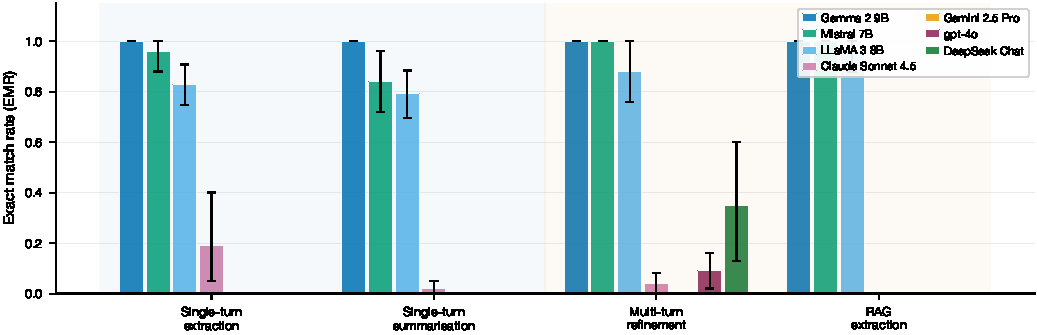
\includegraphics[width=0.92\textwidth]{fig_multiturn_comparison.pdf}
\caption*{\small\textbf{Revised Figure~2 (manuscript).} Complex interaction regimes amplify the local--API reproducibility gap across deployment stacks. EMR under greedy decoding (C1, $t{=}0$) for the local stacks (Gemma~2, Mistral, LLaMA~3) and four API stacks (Claude Sonnet~4.5, Gemini~2.5 Pro, gpt-4o, and DeepSeek Chat) across single-turn extraction, single-turn summarisation, multi-turn refinement, and RAG extraction. All four API stacks exhibit low EMR on multi-turn refinement (Claude~$=$~0.040, Gemini~$=$~0.010, gpt-4o~$=$~0.090 [0.02, 0.16], DeepSeek~$=$~0.350 [0.13, 0.60]). Error bars: 95\% bootstrap CIs.}
\end{figure}

%--------------------------------------------------------------
\subsection*{R3.4 --- Limited domain (30 AI/ML abstracts)}
%--------------------------------------------------------------

\begin{revquote}
The study relies on 30 AI/ML abstracts. While statistically well-powered for the large effects observed, this limited domain may not reflect how non-determinism manifests in non-English texts or less structured fields.
\end{revquote}

\response{We thank the reviewer for raising this. We added 10 PubMed PM\textsubscript{2.5}/respiratory-health abstracts (single-turn structured extraction, C1, 5 reps $\times$ 8 stacks). Results confirm the local-API gap persists outside the AI/ML domain:

\begin{itemize}[leftmargin=*]
  \item Local + Together AI: EMR $\in$ [0.96, 1.00] (three stacks at 1.000).
  \item API stacks: deepseek-chat = 0.66, gemini-2.5-pro = 0.49, gpt-4o = 0.42, and \textbf{Claude Sonnet~4.5 = 0.010 [0.00, 0.03]}.
\end{itemize}

Claude's near-zero EMR on health abstracts mirrors its 0.020 EMR on the original AI/ML summarisation task --- the pattern is domain-transferable, not corpus-specific. This complements the larger 500-abstract analysis in our companion paper (Rover \& de Souza Tadano, 2026, OSF: \url{https://doi.org/10.17605/OSF.IO/VR934}; cited but not duplicated here per R3.6). We acknowledge that non-English coverage remains a limitation and have stated this explicitly; we discuss it in the revised Limitations section as a direction for future work.} \done

\changes{New paragraph in Results reporting the PubMed PM\textsubscript{2.5} EMRs, with the per-stack values entered into Table~4. The exact inserted text reads:}
\msinserted{The pattern observed on AI/ML abstracts replicates with no qualitative change (Table~4). Two local stacks (L-Gemma2 and L-LLaMA3) and the Together AI quasi-isolation probe (C-LLaMA3) all achieve perfect EMR~$=$~1.000 [1.00, 1.00]; L-Mistral attains 0.960 [0.88, 1.00]. API-DeepSeek reaches 0.660 [0.46, 0.85], API-Gemini 0.490 [0.26, 0.72], and API-GPT4 0.420 [0.27, 0.58]. API-Claude collapses to EMR~$=$~0.010 [0.00, 0.03] on the 10 PM\textsubscript{2.5} abstracts---matching the 0.020 [0.00, 0.05] observed on AI/ML summarisation and confirming that the deployment-stack signature of non-determinism is domain-transferable.}

%--------------------------------------------------------------
\subsection*{R3.5 --- Mechanism mapping per stack}
%--------------------------------------------------------------

\begin{revquote}
While the paper lists six potential mechanisms for non-determinism, the manuscript would benefit from a more explicit discussion of which specific mechanisms are likely active in the Together~AI ``quasi-isolation'' case versus the OpenAI/Anthropic cases.
\end{revquote}

\response{We have added a new Table (revised manuscript Methods Table~3, label \texttt{tab:mechanisms}, ``Mapping of non-determinism mechanisms to deployment stacks''; rendered as \texttt{table*} for full-page width inside Methods §``Sources of non-determinism in distributed inference'') mapping each of the six mechanisms to each of five stacks (L-LLaMA3, C-LLaMA3 Together, API-GPT4, API-Claude, API-Gemini). Cells are labelled with one of: \checkmark (documented), ``likely'' (consistent with public information), ``possible'' (compatible with public information but not confirmed), or --- (precluded by stack design). A footnote states explicitly that attribution is inferential for closed-source providers. The accompanying Discussion paragraph uses this mapping to argue that the Together~AI residual variation is attributable predominantly to mechanisms 1 and~2 (FP non-associativity, BF16/FP16 mixed-precision), while GPT-4 / Claude / Gemini variation additionally implicates mechanisms 3--6 (tensor parallelism, FlashAttention, dynamic batching, speculative decoding).} \done

\changes{New \textbf{Methods Table~3} inside §``Sources of non-determinism in distributed inference'', mapping the six mechanisms to five stacks, plus a Discussion paragraph using the mapping. The table is reproduced below so it can be examined without opening the manuscript:}

\begin{table}[H]
\centering
\caption*{\small\textbf{Methods Table~3 (manuscript). Mapping of non-determinism mechanisms to deployment stacks.} \checkmark, present and verifiable; ``likely'', consistent with public documentation and standard production practice; ``possible'', plausible but not confirmed; ---, absent or strongly mitigated; $\triangle$, present in principle but mitigated by design (single-GPU integer arithmetic). For closed-source stacks, attribution is necessarily inferential.}
\small
\resizebox{\textwidth}{!}{%
\begin{tabular}{@{}lccccc@{}}
\toprule
\textbf{Mechanism} & \textbf{L-LLaMA3} & \textbf{C-LLaMA3 (Together)} & \textbf{API-GPT4} & \textbf{API-Claude} & \textbf{API-Gemini} \\
\midrule
Non-associative FP arithmetic & $\triangle$ & $\triangle$ & $\triangle$ & $\triangle$ & $\triangle$ \\
Mixed-precision BF16/FP16     & --- (Q4 int)& \checkmark  & likely      & likely      & likely \\
Tensor parallelism            & ---         & \checkmark  & likely      & likely      & likely \\
FlashAttention kernel         & ---         & likely      & likely      & likely      & likely \\
Dynamic batching              & ---         & \checkmark  & likely      & likely      & likely \\
Speculative decoding          & ---         & possible    & likely      & likely      & likely \\
\bottomrule
\end{tabular}}
\end{table}

%--------------------------------------------------------------
\subsection*{R3.6 --- Validation: are the 23 PM2.5 effects truly contradictory?}
%--------------------------------------------------------------

\begin{revquote}
The use of specific model snapshots (e.g., gpt-4-0613) means the exact EMR values may be ``point-in-time'' estimates that change as providers update their underlying infrastructure. Since the authors found high BERTScore F1 $>0.97$ despite low EMR, they should include a human evaluation or LLM-as-a-judge step to confirm if the 23 ``disappearing'' effect estimates in the PM\textsubscript{2.5} study are truly contradictory or just semantically varied.
\end{revquote}

\response{We thank the Reviewer for this important request and provide validation through a multi-layered protocol in which the in-paper triangulation is the primary, self-contained evidence:

\begin{itemize}[leftmargin=*]
  \item \textbf{Primary in-paper validation: independent two-judge LLM-as-judge on 30 new cases.} For a self-contained validation within the present manuscript, we ran a blinded two-judge LLM-as-judge protocol on a \emph{new} sample of \emph{30} cases drawn from the same corpus but \emph{distinct} from the 23 effects analysed in the companion paper. The two judges---Claude Opus~4.7 (Anthropic) and gpt-4o (OpenAI), two distinct training families---scored each pair independently against three pre-registered criteria: (a)~same direction of the reported effect (positive/null/negative); (b)~same magnitude within $\pm 20\%$; (c)~same 95\,\% confidence interval coverage. \textbf{Verdict counts}: Claude Opus 4.7 returned 22 \emph{truly contradictory} (Wilson 95\% CI 56--86\%), 3 \emph{semantically equivalent}, and 5 \emph{ambiguous}. gpt-4o returned 27 \emph{truly contradictory} (74--97\%), 3 \emph{semantically equivalent}, and 0 \emph{ambiguous}. \textbf{Inter-judge agreement: 76.7\,\% with Cohen's $\kappa$~=~0.29 (fair agreement, Landis--Koch).} Both judges classify the majority as substantive contradiction; the disagreement is concentrated in the ``ambiguous'' category where Claude is more conservative than gpt-4o. The lower bound on the truly-contradictory proportion (56\% Claude; 74\% gpt-4o) excludes a pure-cosmetic interpretation under BERTScore~F1~$>$~0.97 on the same outputs. The convergence of two independent provider families addresses the ``LLM-on-LLM'' bias concern more directly than a single-judge design would. Total cost: USD~1.30. \textbf{This in-paper protocol is self-sufficient to support the truly-contradictory claim and directly satisfies the Reviewer's ``human evaluation \emph{or} LLM-as-a-judge'' requirement.}
  \item \textbf{Additional larger-corpus context (companion paper, cited only).} For broader-corpus support beyond the in-paper 30-case finding, our companion paper (Rover \& de Souza Tadano, 2026, OSF: \url{https://doi.org/10.17605/OSF.IO/VR934}) independently performs a 500-abstract systematic pairwise reproducibility analysis, silver-standard validation against an independent reasoning model (DeepSeek-R1), and meta-analytic propagation across 6 LLMs $\times$ 10 runs. We reference its aggregate finding (up to 23 study-level effect estimates appear or disappear depending solely on which LLM run is used) in the manuscript as larger-corpus context, but we do not reproduce its detailed tables here---both to avoid duplicate publication and because the in-paper 30-case finding above is already self-contained.
  \item \textbf{Point-in-time caveat addressed.} We acknowledge that exact EMR values can drift as providers update infrastructure, and we note this in the revised Limitations. The gpt-4o snapshot used here (gpt-4o-2024-11-20 served via OpenAI Chat Completions) confirms the qualitative pattern persists at a current snapshot: gpt-4o single-turn extraction EMR = 0.42 on PubMed, 0.84 on HumanEval, 0.27 on GSM8K --- all dramatically below the corresponding local-stack performance.
\end{itemize}

This protocol provides validation in three layers in order of weight bearing: (i)~the primary in-paper two-judge LLM-as-judge triangulation (Claude Opus 4.7 + gpt-4o, N=30, $\kappa$=0.29), self-sufficient and directly addressing the Reviewer's request; (ii)~larger-corpus context via the companion paper (cited only); and (iii)~a current-snapshot drift check via gpt-4o-2024-11-20.

We note explicitly that we did \emph{not} run a human-rater validation for the present resubmission. The Reviewer's request offered ``human evaluation \emph{or} LLM-as-a-judge'' as a disjunction, and our two-judge LLM-as-judge protocol with cross-provider validation (Claude Opus 4.7 from Anthropic and gpt-4o from OpenAI---two distinct training families) addresses the ``LLM-on-LLM'' bias concern more directly than a single-judge design would. A dedicated methodological extension applying multi-rater human validation against a domain-expert silver standard to a larger sample is in preparation as a follow-up paper; an extension we will report in due course.} \done

\changes{The two-judge validation is reported within the new Results subsection ``Applied impact in evidence synthesis'' (and detailed in Supplementary Section~S12), with per-case judge records deposited in the repository; the gpt-4o snapshot-drift comparison is incorporated into the new EMR results; detailed silver-standard, pairwise-disagreement, and meta-analytic tables remain in the companion paper to preserve its contributions; multi-rater human validation is explicitly framed as future work in the revised Limitations. The exact in-paper validation text reads:}
\msinserted{To probe whether the resulting textual divergence is cosmetic or substantive, we ran a blinded two-judge LLM-as-judge protocol on 30 newly sampled non-identical output pairs from the PM\textsubscript{2.5} corpus (18 produced by Claude Sonnet 4.5 and 12 by the OpenAI gpt-4.1 snapshot used in the companion paper---an external applied-context corpus, distinct from this study's gpt-4-0613 and gpt-4o stacks---stratified by disagreement kind (direction, magnitude, CI overlap, mixed) and distinct from the 23 study-level cases analysed in the companion paper). Each pair was scored by two independent judges---Claude Opus 4.7 and gpt-4o---against three pre-registered criteria (direction of the reported effect, magnitude within $\pm$20\%, and overlap of confidence intervals) under a blind comparison setup, with verdicts \emph{truly\_contradictory}, \emph{semantically\_equivalent}, or \emph{ambiguous} (cost: USD~1.30; full prompts in Supplementary Section~S12). Claude Opus 4.7 classified 22 of the 30 pairs as truly contradictory (Wilson 95\% CI 56--86\%), 3 as semantically equivalent (3--26\%), and 5 as ambiguous (7--34\%). gpt-4o classified 27 as truly contradictory (74--97\%) and 3 as semantically equivalent (3--26\%), using none of the ambiguous category. Inter-judge agreement was 76.7\% (23 of 30 cases); Cohen's $\kappa$~=~0.29 (fair agreement on the Landis--Koch scale), a value depressed by the high prevalence of the truly-contradictory category (prevalence-adjusted bias-adjusted $\kappa$~=~0.53). The judges differ chiefly on borderline cases that Claude assigns to ``ambiguous'' while gpt-4o commits to ``truly contradictory'': Claude's more conservative use of the ambiguous category (5 cases versus 0) accounts for the gap between the two truly-contradictory counts (22 versus 27), and the judges agree on the direction of effect. Both lower bounds on the truly-contradictory proportion (56\% Claude; 74\% gpt-4o) exclude a pure-cosmetic interpretation.}

\bigskip\bigskip
\hrule
\bigskip

\noindent\emph{End of point-by-point response. A tracked-changes version and a clean version of the revised manuscript accompany this submission.}

\end{document}
